\documentclass[../main.tex]{subfiles}

\begin{document}
\section{Datasets} \label{sec:datasets}

In this chapter for this master thesis relevant datasets are introduced. All datasets, except the first one which is used as reference to verify implementation details, belong to the domain of drug discovery.

\subsection{Covertype} \label{ssec:covertype}

The dataset consist of 581012 samples describing forest cover types within a national park in Colorado US. The dataset consists of 54 features with 10 of them being numerical and 44 binary. The setting is a multi-class classification task for 7 different forest cover types. The dataset was collected and created in 1998 \cite{blackard_comparative_1998} and is freely available within the University of California Irvine (UCI) dataset collection \cite{covertype_uci_nodate}. 

The dataset is used within this master thesis to verify the implementation of TabNet based on the achieved performance before any subsequent experiments. The forest cover type dataset was used within the TabNet paper \cite{arik_tabnet_2020} as one dataset for which the architecture achieved better performance than other techniques such as GBDT or DNN. 

Additionally Google published a repository exactly and only for this dataset testing TabNet \cite{noauthor_google-researchtabnet_nodate} including the splitting process into training, validation, and testing part as well as random seeds used. The same splits (54\% training, 26\% validation, 20\% testing) were used within this master thesis.

\subsection{Blood-Brain-Barrier Penetration Dataset} \label{ssec:bbbp}


The dataset consists of about 2000 molecules for each of which the characteristic whether the individual molecule can penetrate the blood-brain-barrier (BBB) or not is known. The BBB describes a membrane that separates circulating blood from extracellular fluid within the brain to protect the brain from intruding substances. Large molecules within drugs can not pass it and only about 2\% of small molecules can. Therefore in case the passing of the barrier is desired within drug discovery finding such molecules which are able to penetrate those membrane is difficult. On the other hand for toxicology of newly developed drugs it is critical to test for penetration of the BBB \cite {martins_bayesian_2012}.

\subsection{Beta-Secretase 1 Dataset} \label{ssec:bace}

The Beta-secretase 1 (BACE) dataset consists of molecules with binding results, in quantitative form for regression and in binary form for classification, for the human Beta-secretase 1 (BACE-1). The Beta-secretase 1 is an enzyme in humans, encoded in the BACE1 gene, which is mainly expressed within neuron cells. This enzyme plays a major role in the generation of amyloid-$\beta$ peptides in neurons and are the main components in amyloid plaques which are found in human brains with Alzheimer disease (AD). Following the amyloid hypothesis, finding drugs which are BACE inhibitors in theory may prevent or at-least slow down AD \cite{pradeepkiran_protective_2020}.

The BACE dataset consists of about 1500 molecules represented as SMILE strings with binary classification whether being a BACE inhibitor (1) or not (0). Additionally the quantitative inhibitor property represented as $IC_{50}$ value and the 2D structures of molecules are available \cite{subramanian_computational_2016}. In this master thesis only the qualitative inhibit property is used in a binary classification setting. 

The dataset is publicly available within the MoleculeNet dataset collection \cite{wu_moleculenet_2018}.

\subsection{Human Immunodeficiency Viruses Dataset}

The human immunodeficiency viruses (HIV) datasets consists of more than 40000 molecules describing their ability to inhibit HIV replication. HIV causes acquired immunodeficiency syndrome (\acs{aids}) which causes failure of the immune system and per average leads to death within 9 to 11 years\cite{noauthor_hiv_2021}. The dataset was introduced by the drug therapeutics program for AIDS antiviral screening \cite{noauthor_aids_nodate}.

The original HIV dataset consists of 3 categories being inactivity (not inhibiting), activity and moderate activity (inhibiting). The later two categories are combined leading to a binary classification task. Molecules are represented as smile strings. The dataset is publicly available within the MoleculeNet dataset collection \cite{wu_moleculenet_2018}.

\subsection{Side Effect Resource Dataset}

The side effect resource dataset (SIDER) consists of developed drugs available on the market with reported adverse drug reactions (ADR) during clinic trials. The datasets consists of over 1400 marketed drugs represented as smile strings with their reported side effect\cite{kuhn_sider_2016}. Beside the prepared dataset the side effect resource database exists\footnote{http://sideeffects.embl.de/}. 

The dataset publicly available within MoleculeNet \cite{wu_moleculenet_2018} reports 27 categories for side effect represented as binary targets which lead to a multi target binary classification task. Per category 1 indicates that the side effect has been reported for corresponding drug and 0 if not has been reported. 
% The 27 binary ategories are:

% \begin{enumerate}
% 	\item \emph{Hepatobiliary disorders}
% 	\item \emph{Metabolism and nutrition disorders}
% 	\item \emph{Product issues}
% 	\item \emph{Eye disorders}
% 	\item \emph{Investigations}
% 	\item \emph{Musculoskeletal and connective tissue disorders}
% 	\item \emph{Gastrointestinal disorders}
% 	\item \emph{Social circumstances}
% 	\item \emph{Immune system disorders}
% 	\item \emph{Reproductive system and breast disorders}
% 	\item \emph{Neoplasms benign, malignant and unspecified (incl cysts and polyps)}
% 	\item \emph{General disorders and administration site conditions}
% 	\item \emph{Endocrine disorders}
% 	\item \emph{Surgical and medical procedures}
% 	\item \emph{Vascular disorders}
% 	\item \emph{Blood and lymphatic system disorders}
% 	\item \emph{Skin and subcutaneous tissue disorders}
% 	\item \emph{Congenital, familial and genetic disorders}
% 	\item \emph{Infections and infestations}
% 	\item \emph{Respiratory, thoracic and mediastinal disorders}
% 	\item \emph{Psychiatric disorders}
% 	\item \emph{Renal and urinary disorders}
% 	\item \emph{Pregnancy, puerperium and perinatal conditions}
% 	\item \emph{Ear and labyrinth disorders}
% 	\item \emph{Cardiac disorders}
% 	\item \emph{Nervous system disorders}
% 	\item \emph{Injury, poisoning and procedural complications}
% \end{enumerate}

% \subsection{Tox21}

% Load Tox21 dataset

% The “Toxicology in the 21st Century” (Tox21) initiative created a public database measuring toxicity of compounds, which has been used in the 2014 Tox21 Data Challenge.53 This dataset contains qualitative toxicity measurements for 8014 compounds on 12 different targets, including nuclear receptors and stress response pathways.

\subsection{Human Ether-à-go-go-Related Gene Dataset} \label{ssec:herg_dataset}

The human ether-a-go-go related gene (hERG) dataset encodes a protein $K_v11.1$ relevant for the potassium ion channel within the heart. This channel mediates the electrical current flow of ions and helps regulating heart beats. When the ability of this channel to conduct electrical current is inhibited or effected this can lead to fatal disorder of the heart and subsequent to death. 

Therefore within drug discovery molecules are regularly tested for their hERG characteristic. The dataset used within this master thesis consists of about 8000 molecules represented as SMILES string. For each molecule the hERG activity, 1 for blocking, 0 for non-blocking/decoy molecule and not further defined (n/d) is given. hERG active molecules are thresholded having $IC_{50} \le 10 \mu M$. The non-blocking or decoy molecules, molecules which are randomly extracted from chemical databases but resemble similarities with known hERG active molecules, are split using different $IC_{50}$ thresholds. This results into 6 targets for non-blocking/decoy (0) if $IC_{50}$ above $10, 20, 40, 60, 80, 100$ $\mu M$ respectively and not defined (n/d) if below but above the active threshold ($IC_{50} > 10) \mu M$. This results into a multi binary target classification setting for which not every sample is fully defined for all targets (0, 1, n/d). In this work only the first target is used which in fact is fully defined (0 or 1) for all samples. The dataset is publicly available within the support information of the introducing paper \cite{cai_deep_2019}.
\newline

Furthermore recent work \cite{czodrowski_herg_2013} identified common motifs within hERG active and inactive molecules using maximum common substructures analysis on publicly available hERG data. Using various source data on hERG activity, which were collected using functional and binding assays and with two different thresholds ($1 \mu M$, $10 \mu M$) for $IC_{50}$ binding affinity, 15 unique relevant substructures could be identified. Only complete ring structures and motifs with at-least 5 heavy non hydrogen atoms were considered. Some identified substructures were found within hERG active and inactive molecules. 
In table \ref{tbl:hergophores} all 15 substructures including their smile strings, IUPAC names, drawings and hERG active and inactive are shown. 5 substructures are exclusively found in hERG active molecules, 6 exclusively in hERG inactive molecules and 4 were found in both. The original differentiation between assay type and thresholds is not represented anymore, for those details including the number of matches for each substructure within the molecules refer to original authors work \cite{czodrowski_herg_2013}. 
\newline

Following similar approach as done in the work by Schimunek J. et al. \cite{schimunek_poster_2021} this master thesis uses the described relevant substructures, especially ones which are exclusively related to hERG active, as a baseline. Refer to section \ref{sssec:evaluation_methodology} for details.

\begin{table}[H]
	\centering
	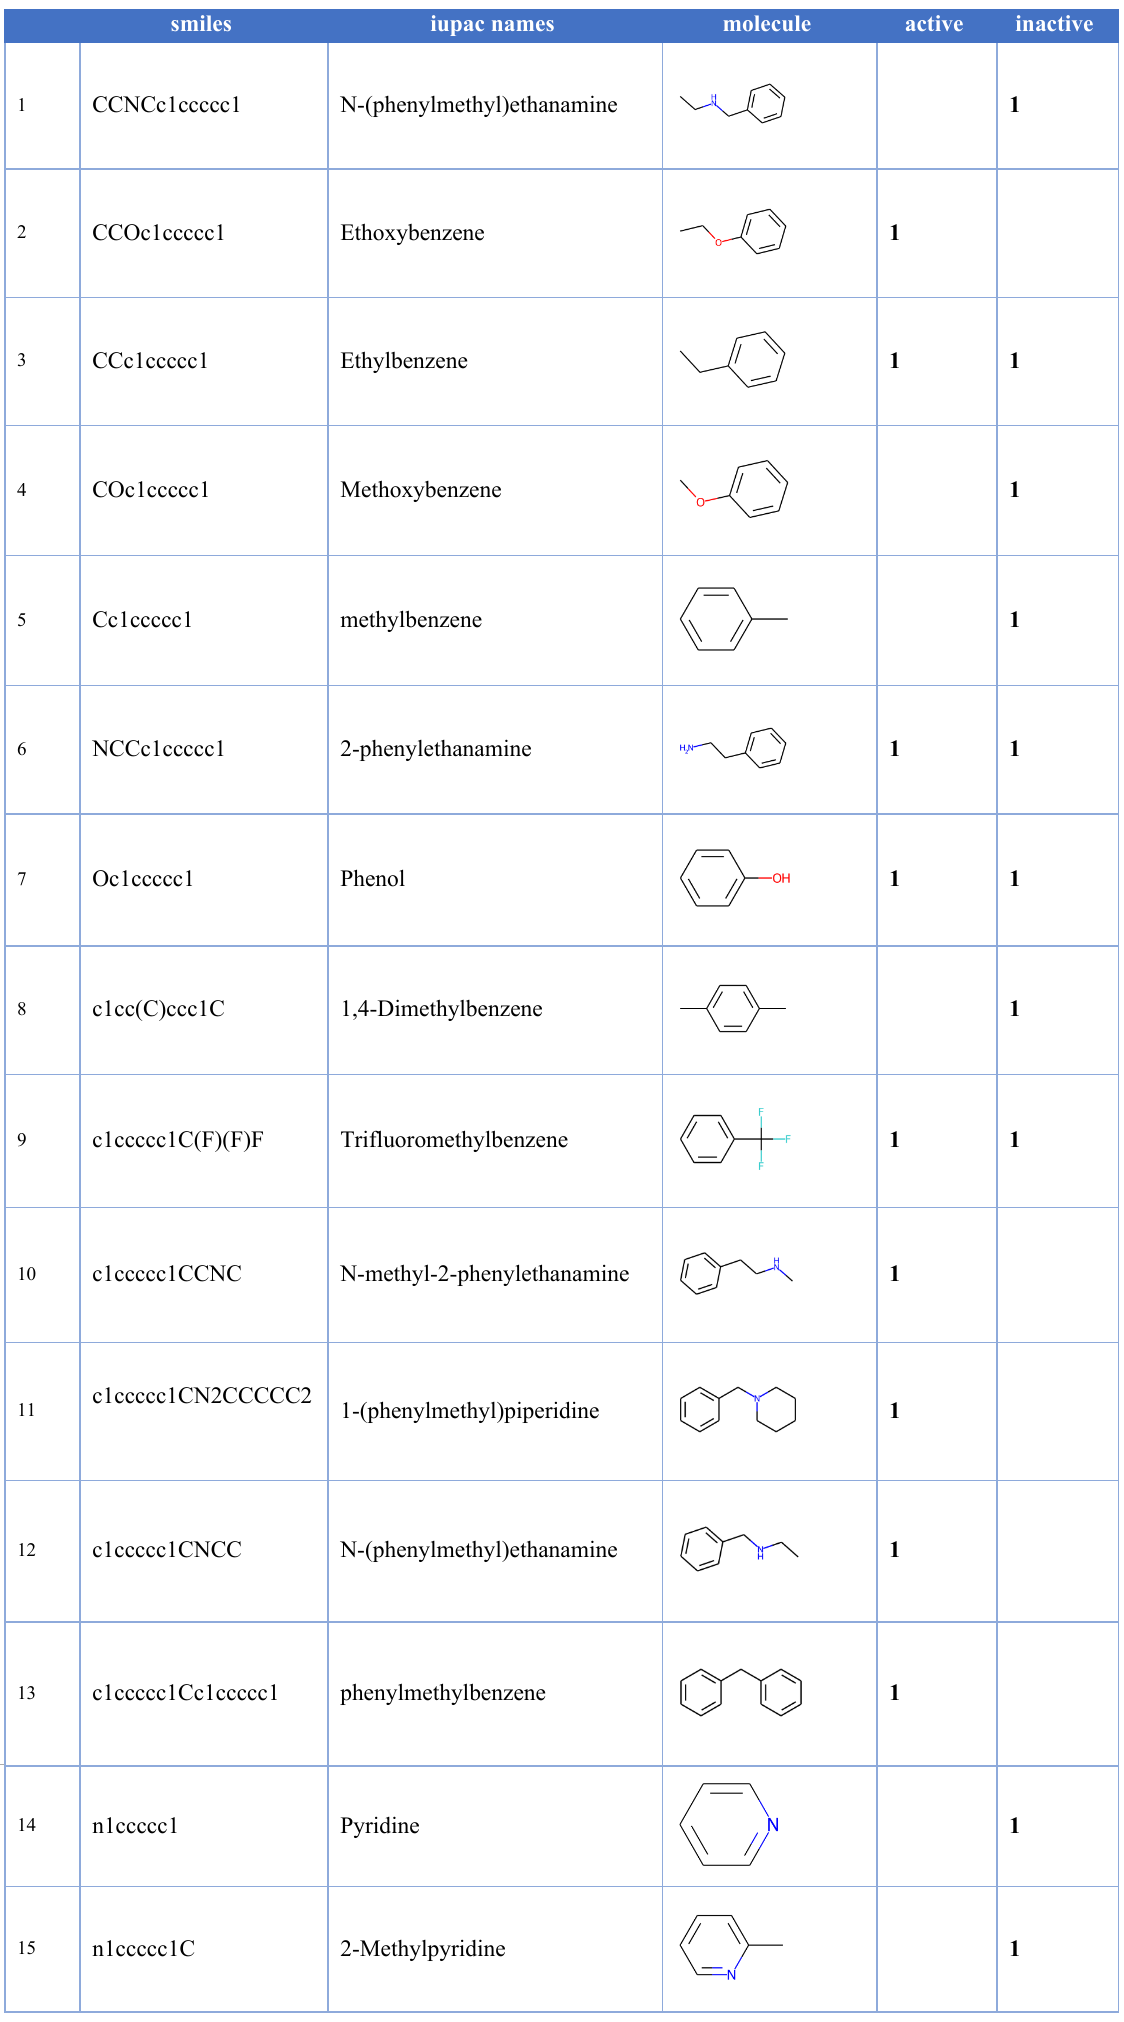
\includegraphics[width=0.8\textwidth]{hergophores}
	\caption{hERG identified relevant substructures including the SMILE string, IUPAC chemical name, hERG active and inactive status \cite{czodrowski_herg_2013}}
 	\label{tbl:hergophores}	
\end{table}
     
\end{document}